\begin{section}{Introduction}
Fair and efficient allocation of link bandwidth is an important constraint for packet scheduling in a switch. Although the Generalised Processor Sharing (GPS) algorithm ensures both fairness and efficiency, it is highly impractical. In this simulation, the Weighted Fair Queueing algorithm for packet scheduling is implemented and tested. Weighted Fair Queueing achieves fairness and efficiency equivalent to GPS on a comparatively larger time scale. 
\end{section}


\begin{section}{Implementation}
Each packet source generates packets with uniformly distributed lengths and exponential inter-arrival times. Thus each packet source is essentially a Poisson source. On adding a newly generated packet to the queue, if size permits, the round number and finish numbers of the flow are updated. The packet are stored in a priority queue according to the finish numbers so that the packet with the smallest finish number can be easily selected for transmission. \\
Each packet source is implemented as an independent thread and wakes up the scheduler when it generates a packet. After the required round and finish number book-keeping, the scheduler inserts the packet in the queue and wakes up the transmitting thread. If the transmitting thread is free, it selects the next packet and starts transmission. \\
Additionally there is a metric thread that wakes up after a fixed number of time units and computes the Jain's fairness metric and relative fairness bound.
\end{section}

\begin{section}{Results}


The bandwidth allocation for 8 and 16 packet sources are depicted below. For both scenarios, two cases are considered, Case-1 with equal weights, and Case-2 is with unequal weights. The blue bars represent the weighted fair allocation and the orange bars depict the allocation acheived by the simulation. Clearly, the simulation nearly achieves the optimal allocation. This experiment was conducted with high buffer size, and lower processing rate (as compared to packet generation rate) to not only minimise the effects of handling packet drop, but also have enough pending packets of every flow to achieve relative fairness. 

\begin{figure}[h] % Positioning option: h (here)
    \centering
    \begin{subfigure}[b]{0.45\textwidth}
        \centering
        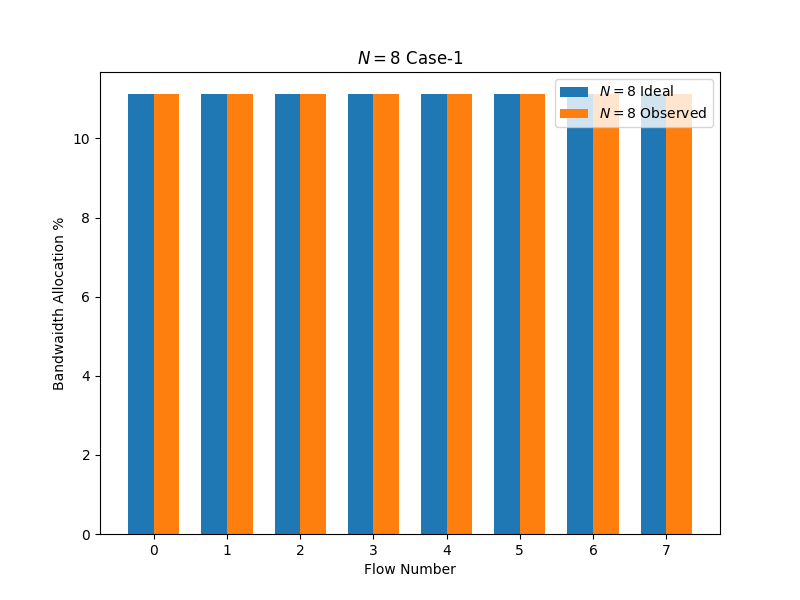
\includegraphics[width=\textwidth]{figures/fig1/N=8_1.png} % Replace with your first image file
        \label{fig:image1}
    \end{subfigure}
    \hfill
    \begin{subfigure}[b]{0.45\textwidth}
        \centering
        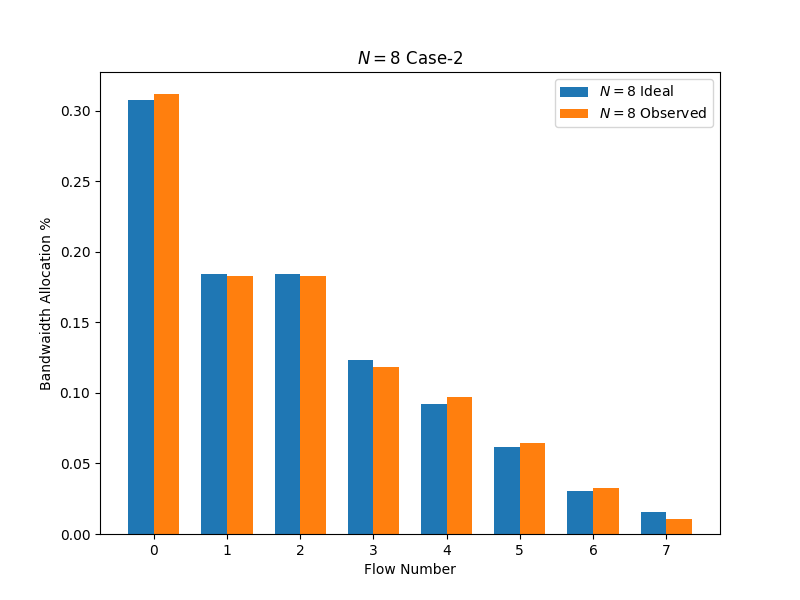
\includegraphics[width=\textwidth]{figures/fig1/N=8_2.png} % Replace with your second image file
        \label{fig:image2}
    \end{subfigure}
    \caption{$N=8$ Performance Graphs}
    \label{fig:two_images}
\end{figure}


\begin{figure}[h] % Positioning option: h (here)
    \centering
    \begin{subfigure}[b]{0.46\textwidth}
        \centering
        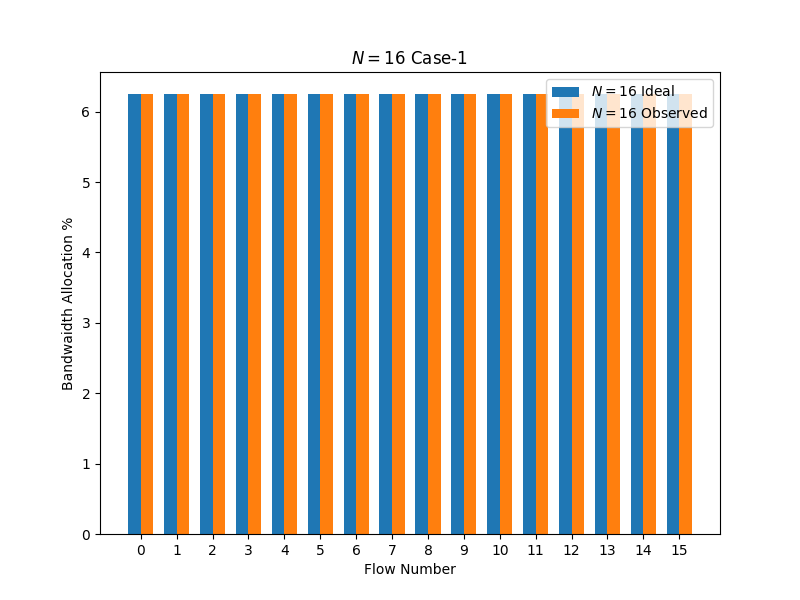
\includegraphics[width=\textwidth]{figures/fig1/N=16_1.png} % Replace with your first image file
        \label{fig:image1}
    \end{subfigure}
    \hfill
    \begin{subfigure}[b]{0.46\textwidth}
        \centering
        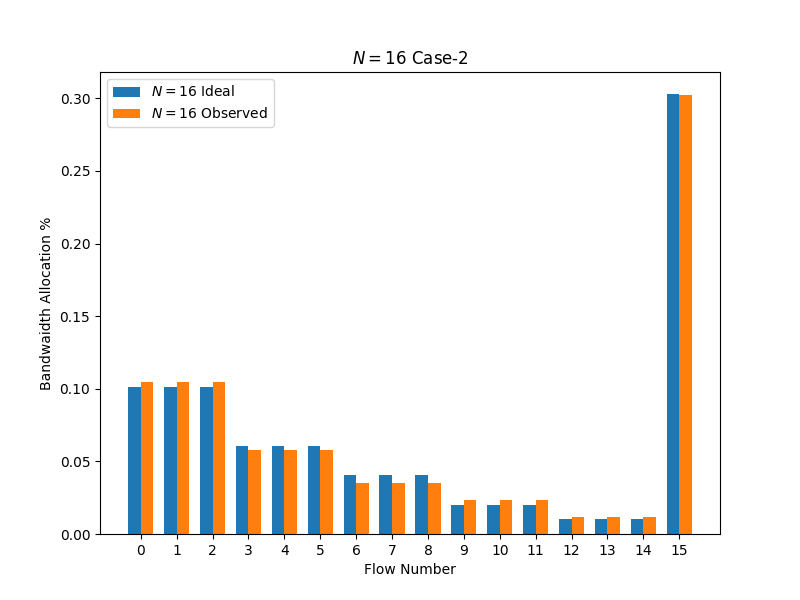
\includegraphics[width=\textwidth]{figures/fig1/N=16_2.png} % Replace with your second image file
        \label{fig:image2}
    \end{subfigure}
    \caption{$N=16$ Performance Graphs}
    \label{fig:two_images}
\end{figure}
\end{section}

\begin{section}{Performance \& Analysis}
    \begin{subsection}{Contributing Effects}
        Due to the peculiar choice of dropping packet with the smallest finish number (as mentioned in the question), the following effects influence the weighted fairness:
        \begin{itemize}
            \item \textbf{Low buffer space effect}: Because of low buffer space, the flows with lower weight, but higher packet generation rate will hog the queue, not allowing the higher priority flows to even enter the queue despite having lower finish numbers.
            \item \textbf{Removing smallest finish number effect}: When there is a packet from a flow, the Head-of-Line packet for that flow is deleted. This adversely affects the bandwidth alloted to that flow. Thus, if the packet generation rate of a flow is high, it leads to deletion of more HOL packets for that flow, causing a lesser bandwidth being allotted to it. In conclusion, with smallest finish number packet drop policy, flows with high packet generation rate suffer more. 
        \end{itemize} 
    \end{subsection}

    \begin{subsection}{Fairness \& Weighted Fairness}
        As seen in the results section, WFS acheives the optimal weighted-fair allocation for every flow. Thus, we have verified that WFS is a practical algorithm that achieves fairness in the long run.
    \end{subsection}

    \begin{subsection}{Delay}
        WFS minimises the delay because of the following two factors:
        \begin{itemize}
            \item Work-Conservation: WFS is work conserving. That is, the output link is never inactive when there are waiting packets. This guarantees that the queueing is not introducing any extra delay in the packets.
            \item Shorter Length First: Since the finish number of a longer packet will be higher (because of the \texttt{length / weight} term), it will be placed lower in the queue, and will be scheduled later. One can draw parallels between this mechanism and the shortest job first case in process scheduling, where the shortest jobs are selected first to minimise average waiting time.  
        \end{itemize}
    \end{subsection}

    \begin{subsection}{Time Complexity}
        The priority queue in the simulator operates at $O(\log q)$ for every insert or delete, where $q$ is the size of the queue. Mutex locks and condition variables are used to provide mutual exclusion without significant overheads, like spinning. The time unit is set to $100ms$ to provide sufficient time for all operations in a time unit to complete. Further, at start, the program approximates and prints the expected time to completion, for the input parameters. 
    \end{subsection}
\end{section}

